\section{Ergebnisse}
In diesem Kapitel werden die Ergebnisse des Projektes vorgestellt. Dabei werden sowohl der Verlauf der Implementierungsphase als auch die finalen Ergebnisse behandelt. Zunächst wurde ein Prototyp entwickelt, der die wesentlichen Funktionalitäten des Modells und der Spielumgebung beinhaltet, um sicherzustellen dass das Vorhaben im Rahmen der Vorgaben umsetzbar ist und, um Einblicke in möglichen Problemstellungen des Projektes zu erhalten. Danach wurde der Prototyp Stück für Stück erweitert, bis schließlich das komplette Spiel mit allen Funktionalitäten umgesetzt worden ist und das Modell damit trainiert werden konnte.
\subsection{Trainingshistorie}
\subsubsection{Prototype}
Bei dieser Version handelt es sich um den ersten lauffähigen Prototypen der Umgebung. Es ist nur eines der farbigen Felder (das gelbe) in der Spielumgebung implementiert worden. Das Modell kann mithilfe dieser Spielumgebung bereits trainiert werden und erzielt zum Teil durchaus passable Punktezahlen.\\

Die folgende Abbildung zeigt das erste erfolgreiche Training des Modells:
\nopagebreak
\begin{figure}[H]
	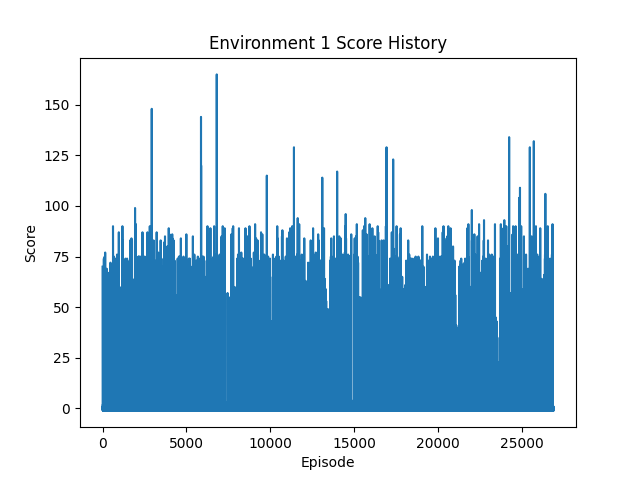
\includegraphics[width=1\textwidth]{Bilder/firstpropertraining} 
	\caption[Erstes erfolgreiches Training]{Erstes erfolgreiches Training\\ Quelle: Eigene Darstellung}
\end{figure}

In der Abbildung erkennt man, dass das Modell innerhalb einer Episode (eines Spiels) des öfteren in einen Punktebereich von 70 zu kommen scheint. Teilweise erzielt das Modell sogar über 150 Punkte. Fragwürdig ist, dass die maximale Punktezahl eigentlich bei 86 liegt und das Modell dennoch zu diesem Zeitpunkt zum Teil Punktewerte erzielt, die höher liegen. Dies ist darauf zurückzuführen, dass die Spielumgebung erzielte Punkte zum Teil mehrfach verwertete und somit mehr Punkte zu erspielen waren, als vorgesehen.\\

Die folgende Abbildung zeigt das erste erfolgreiche Training des Modells in 100 Schritten:
\nopagebreak
\begin{figure}[H]
	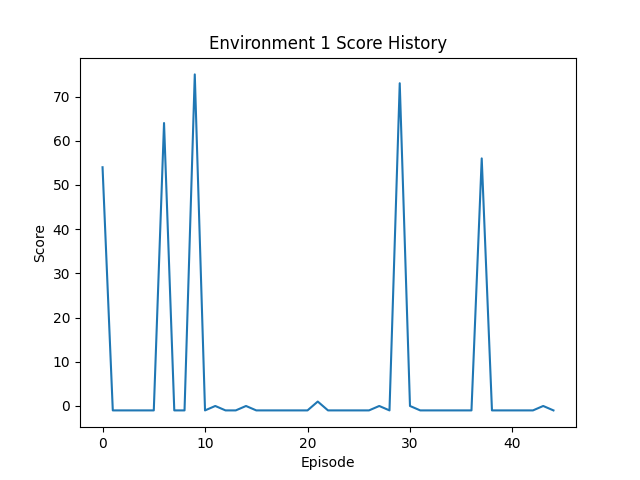
\includegraphics[width=1\textwidth]{Bilder/firstpropertraining100steps} 
	\caption[Erstes erfolgreiches Training 100 Schritte]{Erstes erfolgreiches Training 100 Schritte\\ Quelle: Eigene Darstellung}
\end{figure}

In dieser Abbildung erkennt man, dass das Modell zwar zum Teil eine gute Menge an Punkten erzielt, im Großteil der Spiele allerdings nur null oder einen bis zwei Punkte erzielt. Dies ist darauf zurückzuführen, dass die Spielumgebung bei dieser Version des Projektes das Spiel unverzüglich beendet, wenn eine ungültige Aktion gewählt wird. Daraus kann man schließen, dass das Modell überwiegend ungültige Aktionen wählt, da bei nur 100 Schritten bereits über 40 Spiele abgeschlossen werden. Vorgesehen sind zu diesem Zeitpunkt pro Spiel zehn Spielschritte. Somit wurden über vier mal so viele Spiele abgeschlossen als unter optimalen Bedingungen vorgesehen. Fragwürdig ist hierbei auch, dass das Modell in manchen Episoden mindesten 50/86 Punkten erzielt und in den anderen nur 0 bis 2. Die Punkte werden in Abständen von 10 bis 20 Punkten erspielt, daher handelt es sich hierbei nicht um vereinzelte Erfolge im engeren Sinne.
\subsubsection{Training mit und ohne Aktionsmaske}
Die folgende Abbildung zeigt die erzielten Punkte des Modells ohne Aktionsmaske in 200 Schritten:
\nopagebreak
\begin{figure}[H]
	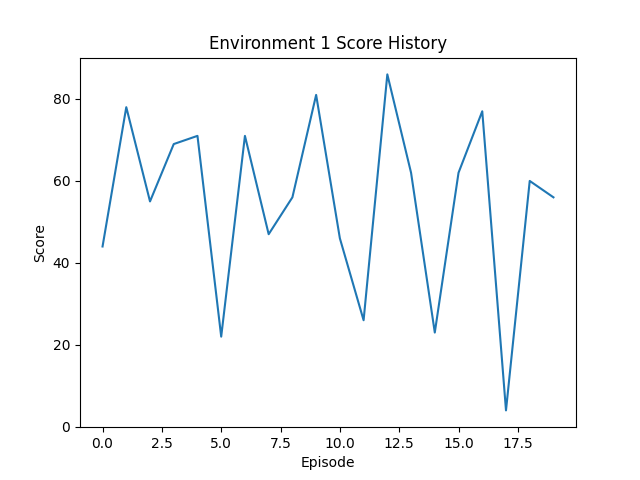
\includegraphics[width=1\textwidth]{Bilder/trainingwithoutcancalation} 
	\caption[Training ohne Aktionsmaske]{Training ohne Aktionsmaske\\ Quelle: Eigene Darstellung}
\end{figure}

Das Training erfolgte zunächst ohne die Verwendung einer Aktionsmaske. Das anfänglicher Verfahren bei dem das Spiel beendet wurde sobald eine ungültige Aktion getätigt wurde stellte sich als nicht geeignet heraus, da das Modell immer wieder ungültige Aktionen wählte, was zum Abbruch vieler Spielrunden führte. Daher wurde eine Trainingsverfahren mit negativer Belohnung bei ungültigen und positiver Belohnung bei gültigen Aktionen gewählt. Diese Belohnungen sind in dieser Abbildung nicht zu sehen, da sie herausgefiltert worden ist. Die Abbildung zeigt nur die aufsummierten Belohnungen, welche 10 oder mehr Punkte betragen. Insgesamt zeigt sich eine verhältnismäßig gute Performance bei der das Modell im Durchschnitt um die 50 Punkte erzielt. Bedenkt man, dass das Maximum bei 86 Punkten liegt ist dieses Ergebnis durchaus vertretbar. Das Modell erzielt somit im Durchschnitt ungefähr 60 Prozent der maximalen Punktezahl.\\

Die folgende Abbildung zeigt die erzielten Punkte des Modells mit Aktionsmaske in 200 Schritten:
\nopagebreak
\begin{figure}[H]
	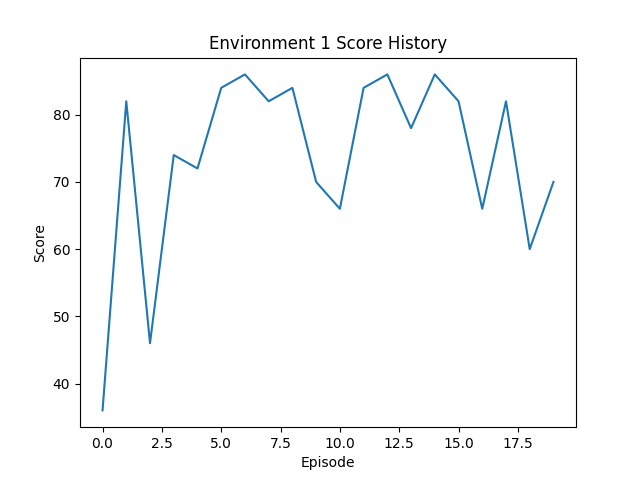
\includegraphics[width=1\textwidth]{Bilder/trainingwithactionmask} 
	\caption[Training mit Aktionsmaske]{Training mit Aktionsmaske\\ Quelle: Eigene Darstellung}
\end{figure}

In dieser Abbildung sieht man, dass die Performance im Gegensatz zu der Variante ohne Aktionsmaske zugenommen hat. Das Modell erzielt im Durchschnitt ungefähr 65 Punkte was einem Zuwachs von circa einem Drittel entspricht. Die erzielten Punkte steigen somit von ungefähr 60 Prozent des Maximums auf 75 Prozent. Zwar lässt sich sagen, dass die Performance des Vorgängermodells passabel war, allerdings erzielt die Variante mit Aktionsmaske ohne größere Umstände ein wesentlich besseres Ergebnis. Deshalb wurde das Projekt ab diesem Zeitpunkt mit Aktionsmaske fortgesetzt.
\subsubsection{Training mit zwei und mit vier Würfeln}
Die folgende Abbildung zeigt die ungültigen Züge einer Spielsimulation von 200 Schritten mit zwei Würfeln:
\nopagebreak
\begin{figure}[H]
	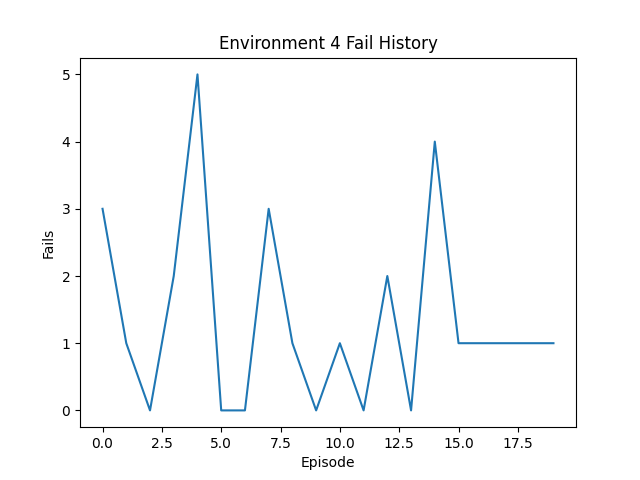
\includegraphics[width=1\textwidth]{Bilder/failswithtwodice} 
	\caption[Ungültige Züge mit zwei Würfeln]{Ungültige Züge mit zwei Würfeln\\ Quelle: Eigene Darstellung}
\end{figure}

In der Abbildung ist zu erkennen, dass das Modell von null bis fünf ungültige Aktionen pro Spiel auswählt. Es ergibt sich ein Durchschnitt von ungefähr 1-2 ungültigen Zügen pro Spiel. Dies sollte nicht auftreten, wenn dem Modell gültige Aktionen zur Verfügung stehen, da die Aktionsmaske dafür sorgt, dass nur gültige Aktionen gewählt werden können. Was passiert allerdings, wenn es keine gültige Aktion gibt? Die Antwort auf die Frage ist: Das Modell wählt eine zufällige Aktion und berücksichtigt die Aktionsmaske nicht. Da nur zwei Würfel zur Verfügung stehen kommt es oft dazu, dass keiner der Würfel zu einem der Felder passt und somit kann keines der Felder ausgefüllt werden. Dadurch steht keine gültige Aktion zur Verfügung und es wird eine ungültige Aktion gewählt.\\

Die folgende Abbildung zeigt die ungültigen Züge einer Spielsimulation von 200 Schritten mit vier Würfeln:
\nopagebreak
\begin{figure}[H]
	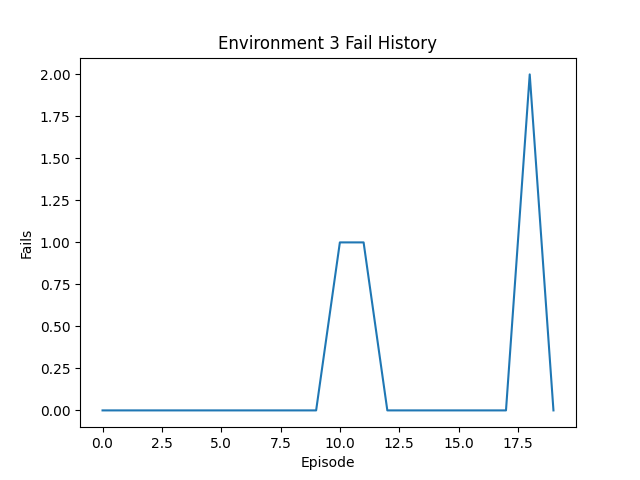
\includegraphics[width=1\textwidth]{Bilder/failswithfourdice} 
	\caption[Ungültige Züge mit vier Würfeln]{Ungültige Züge mit vier Würfeln\\ Quelle: Eigene Darstellung}
\end{figure}

In der Abbildung erkennt man, dass die Anzahl an ungültigen Zügen im Gegensatz zur Variante mit zwei Würfeln drastisch abgenommen hat. Zwar kommt es vereinzelt immer noch zu Fällen bei denen dem Modell nichts anderes übrig bleibt, als eine ungültige Aktion zu wählen, allerdings ist die Wahrscheinlichkeit dafür bei vier Würfeln deutlich geringer.
\subsubsection{Optimiertes Training}
Die folgende Abbildung zeigt die erzielten Punkte des Modells nachdem eine Vielzahl an Optimierungsversuchen durchgeführt worden ist:
\nopagebreak
\begin{figure}[H]
	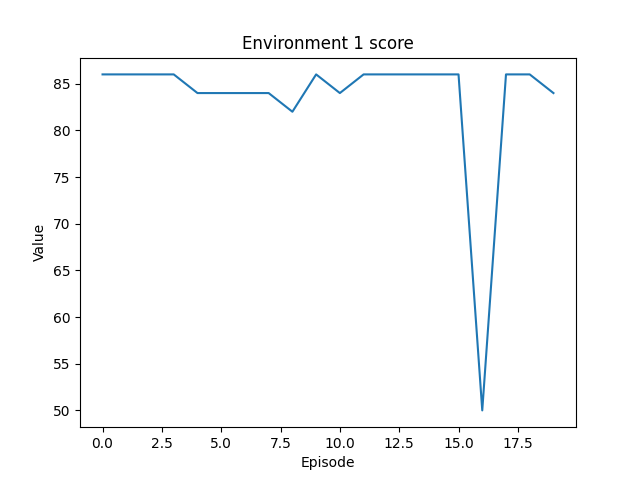
\includegraphics[width=1\textwidth]{Bilder/optimizetraining} 
	\caption[Optimiertes Training]{Optimiertes Training\\ Quelle: Eigene Darstellung}
\end{figure}

Man erkennt, dass das Modell im Durchschnitt etwas mehr als 80 Punkte erzielt hat. Dies ist ein sehr guter Wert, da die maximale Punktezahl bei 86 liegt. Die maximale Punktezahl von 86 Punkten wurde innerhalb der zwanzig Episoden zehn mal erreicht.
\subsection{Erstes Training mit allen Feldern und Boni}
Die folgende Abbildung zeigt die die Ergebnisse des ersten Trainings mit einer Spielumgebung bei der alle farbigen Felder und Boni implementiert worden sind:
\nopagebreak
\begin{figure}[H]
	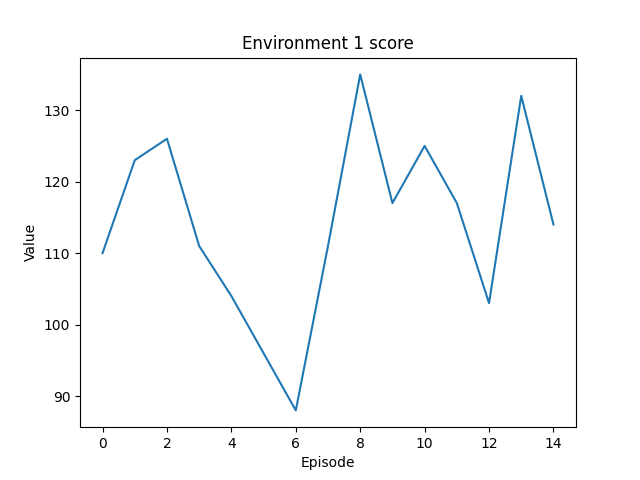
\includegraphics[width=1\textwidth]{Bilder/firsttrainingwithallfields} 
	\caption[Erstes Training mit allen Feldern]{Erstes Training mit allen Feldern\\ Quelle: Eigene Darstellung}
\end{figure}

Man kann erkennen, dass das Modell bereits vertretbare Werte erzielt, allerdings lässt sich an dieser Stelle noch viel optimieren. Im Schnitt erzielt es etwas mehr als 110 Punkte. So viele Punkte erzielt im allgemeinen auch ein Neueinsteiger, der das Spiel kaum kennt. Bei dieser Version des Spiels gibt es auch noch viele Bugs, die dazu führen, dass weniger Punkte erspielt werden, als es unter ordentlichen Bedingungen möglich wäre.
\subsection{Finale Ergebnisse}
\subsubsection{Performance}
Die folgende Abbildung zeigt die erzielten Punkte des Modells nach eingängigem Training:
\nopagebreak
\begin{figure}[H]
	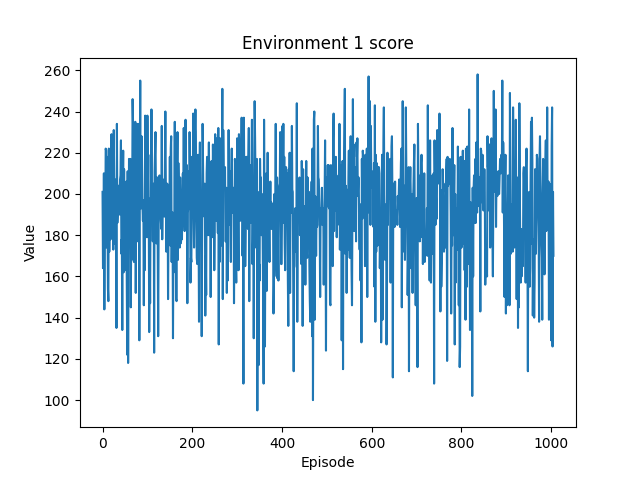
\includegraphics[width=1\textwidth]{Bilder/maskableppo_ganzschoenclever_193avg_v3.1} 
	\caption[Performance 40000 Schritte]{Performance 40000 Schritte\\ Quelle: Eigene Darstellung}
\end{figure}

Das Modell erzielt über mehr als 1000 Episoden eine durchschnittliche Punktezahl von ungefähr 205 Punkten. Das ist beachtlich, da menschliche Spieler in einem Versuch im Durchschnitt lediglich 160 Punkte erzielen konnten. Bei einem weiteren Test über 10000 Schritte liegt Median liegt bei 212 und die durchschnittliche Punktezahl bei 207, was auf ein robustes Modell schließen lässt, da Median und durchschnittliche Punktezahl nah nah beieinander liegen.\\

Die folgende Abbildung zeigt die ungültigen Züge des genannten Modells:
\nopagebreak
\begin{figure}[H]
	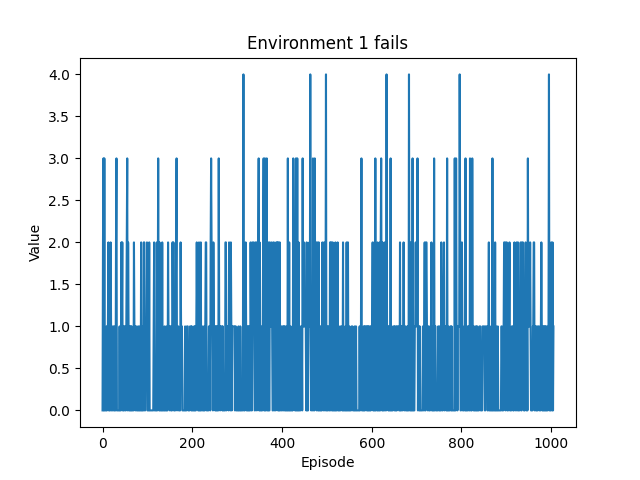
\includegraphics[width=1\textwidth]{Bilder/maskableppo_ganzschoenclever_193avg_v3.1f} 
	\caption[Ungültige Züge 40000 Schritte]{Ungültige Züge 40000 Schritte\\ Quelle: Eigene Darstellung}
\end{figure}

Man erkennt, dass das Modell in den meisten fällen maximal einen ungültigen Zug macht. Teilweise sind noch 2 ungültige Züge pro Episode zu erkennen und noch seltener drei oder vier. Angesichts dessen, dass das Modell pro Spielrunde ungefähr 40 Züge gemacht hat und häufig Würfel bei der Wahl ungültig gemacht werden, ist das ein beachtliches Ergebnis. Das Modell hat gelernt solche Fälle effizient zu vermeiden.\\

Die folgenden beiden Abbildungen zeigen einen Test mit nur 4000 Schritten. Diese Abbildungen sind deutlicher als die mit 40000 Schritten:
\nopagebreak
\begin{figure}[H]
	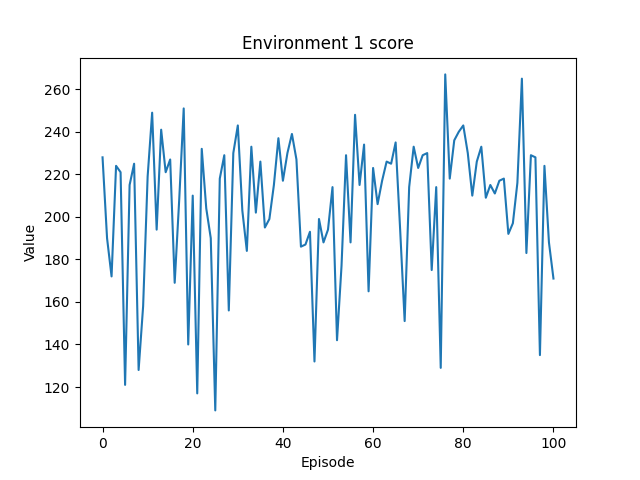
\includegraphics[width=1\textwidth]{Bilder/final4000steps} 
	\caption[Performance 4000 Schritte]{Performance 4000 Schritte\\ Quelle: Eigene Darstellung}
\end{figure}
\begin{figure}[H]
	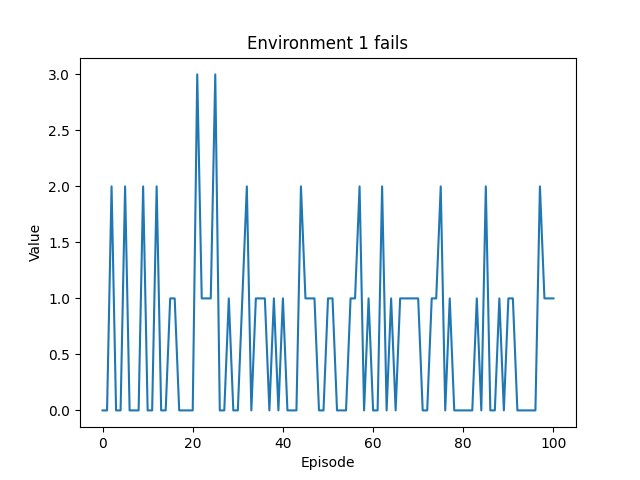
\includegraphics[width=1\textwidth]{Bilder/final4000stepsf} 
	\caption[Ungültige Züge 4000 Schritte]{Ungültige Züge 4000 Schritte\\ Quelle: Eigene Darstellung}
\end{figure}
\subsubsection{Hyperparameter}
Die finalen Hyperparameter sind:

Das Neuronale Netz mit sieben Schichten von jeweils 1024 Neuronen. Ein Gamma von 1. Ein Entropie Koeffizient von 0.1. Eine Lernrate von 0.0006. Eine Clip Range von 0.2. Eine Umgebungsanzahl von 32. Datenpaketen mit 2048 Aktions-Zustands-Paaren, welche jeweils 5 mal verwendet werden und dabei in Batches von 128 Schritten aufgeteilt werden, sowie einem Entropie Koeffizienten für das verfestigen der gelernten Schritte von 0. Das Modell wurde in diesem Prozess zunächst für 2220000 Zeitschritte trainiert. Daraufhin wurde es mit dem Entropie Koeffizient von 0 für weitere 1110000 Zeitschritte trainiert, um das gelernte Verhalten weiter auszunutzen/auszubeuten. Dieser Prozess wurde dann zwei weitere male mit doppelt so vielen Zeitschritten wiederholt. Zunächst betrug die durchschnittliche Punktezahl des Modells annähernd 190, danach 201, danach 205 und nach weiteren Tests schließlich 207 Punkte.

\subsubsection{ChatGPT 4}
ChatGPT [siehe Kapitel 2.2.4] wurde verwendet, um den Prototypen des Projektes bis zu seinem ersten erfolgreichen Einsatz zu implementieren. Dabei hat es sich als besonders nützlich erwiesen, um lauffähigen Code mit den gewünschten, relativ standardmäßigen Methoden zu implementieren. Dies ist gerade bei der Erstellung eines ersten Prototypen vorteilhaft, oder um die Machbarkeit des Projektes zu überprüfen. Im späteren Verlauf wurden von ChatGPT generierte Inhalte nicht mehr direkt übernommen, sondern es wurde nur benutzt, um Auskunft über geeignete oder verwendete Technologien zu geben, Ideen zu sammeln oder Syntax zu erfragen. Auch für diese Aufgaben stellte es sich als sehr nützlich heraus, solange die Fragen nicht zu spezifisch oder komplex waren. Ist die Problemstellung zu komplex oder zu spezifisch, scheint ChatGPT Schwierigkeiten dabei zu bekommen eine vollständige oder geeignete Antwort zu liefern. Außerdem ist die Datenbank des ChatGPT 4 Modells vom September 2021, was den Nutzen für neuere Sachverhalte erschwert.